\chapter{Implementation}
\label{implementation}

\section{System Architecture}
The architecture is shown in the picture below: \\

\begin{figure}[h]
	\centering
  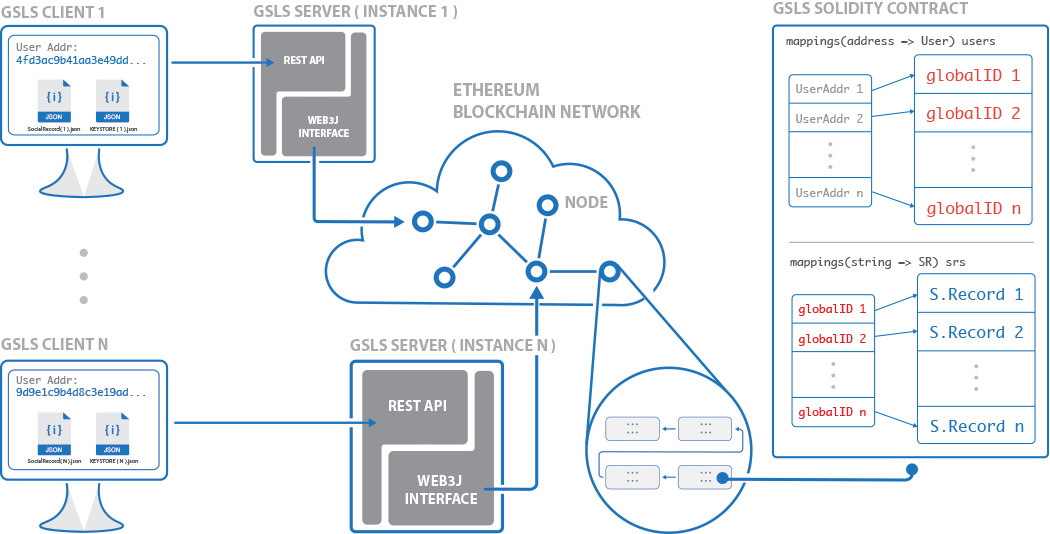
\includegraphics[width=1\textwidth]{gsls-architecture}
	\caption{Basic architecture: n clients communicate with m GSLS server instances. The GSLS instances can interface with the blockchain because each and every of them is holding an Ethereum node. All the operations are referenced to the contract address storing the list of social records.}
	\label{fig1}
\end{figure}

\section{User side}
The client can download the software locally ( directly from the GSLS) from GitHub or wherever it is hosted).
In this case, it is on Electron application running Nodejs on the backend side and React on the front side, where it is possible for a user to login, upload the Ethereum wallet file and the password.
This information is needed to create the row transaction before sending it to the GSLS server.

\subsection{POST /socialrecord \& PUT /socialrecord}
The User can create a new social record or modify an existing one (of course, only if he is allowed to).
When the user clicks on the “submit” Button the following operations are performed:

\begin{list}{},
  \item \textbf{To Address}: convert the address of the receiver (in this case the contract) to Hex
  \item \textbf{Get the Gas price}: the gas price is changing constantly, and in order to set the right amount, it is required to run a get HTTP request to the GSLS server.
  \item \textbf{Gas Limit}: the maximum amount of Gas that the user wants to spend for the transaction to flex.
  \item \textbf{Nonce}: This is a scalar vector equal to the number of the transactions sent from a particular address. It is a value that needs to be always different in order to satisfy the proof of work condition.
  The GSLS Server can retrieve this value, via web3.eth.getTransactionCount(\textit{walletAddress}) and send the result to the user application. Then the nonce is converted to Hex.
  \item \textbf{Data}: The data field is where the meat is. The first 32 bits are reserved for the first 32 bits of the hashed function name (that the user wants to call).
  Then, since in the ABI File, the number of parameters required (and their type) is specified  according to each function : it is possible to grok the bytes needed to append to the data string.
  In the case of creation of a new social record, 2 string parameters are required, which will be converted to hex and appended to the field data space into the string (padding with 0 according to the number of bytes allocated to the string type).
\end{list}

Since the client is the only part of the system allowed to access the wallet file, it must create the mentioned transaction in hexadecimal \textit{style} and sign it with its private key.
The signed transaction can then be sent to the Server via HTTP.

\subsection{GET /socialrecord/:GlobalID}
The get request, used to retrieve the social record for a particular GlobalID, is a simple promise that contacts the server specifying the global id and waiting for the result.

\section{Server}
The GSLS Server can be converted to a REST-ful Server delegated at pulling / pushing social records from / to the blockchain.
The following interfaces are needed:
\subsection{POST /socialrecord \& PUT /socialrecord}
  For a creation of a new social record the following steps are requred:
  \begin{itemize}
    \item GET NONCE \begin{notation}
      TODO
  \end{notation}
    \item The body of the request only contains a signed transaction. The transaction is pushed into the blockchain and the hash of it returned. The hash is useful because starting from that is possible to check the status of the transaction (e.g. on https://ropsten.etherscan.io).
    \item It is possible to create a notification system based on polling, with the client asking for the good or bad result of the operation. It is not possible to send the result in the same HTTP response since it could take more than 90 seconds and therefore time out the request.
  \end{itemize}
  
\subsection{GET /socialrecord/:GlobalID}
The Server receives an HTTP request with one Global ID as parameter. It gets the social record from the blockchain with the help of the ethereum contract function and then it sends it back to the client as an HTTP response.
In this case, it is not required to set up the polling mechanism because the get transaction operates on constant values and therefore does not need to be mined (the mining operation usually takes more time, in Ethereum from 30 seconds to potentially infinite).

\section{Contract}
The contract can be perceived as a class (with constructors and functions) stored in the blockchain.
The mechanism (simplified) is that having the contract stored (with a unique address) in the Ethereum BC and one wallet sending one transaction to the contract address containing the method to call: it is possible to obtain the same output in all the nodes that will receive the transaction.

\subsection{Structures}
In the created social record contract there are 2 structures:

\subsubsection{SR}
\begin{lstlisting}
      struct SR {
          string socialRecord;
          bool exists;
      }
\end{lstlisting}
The social record structure allows storing one string and setting one boolean value to mark if the above mentioned social record is valid.

\subsubsection{User}
\begin{lstlisting}
  struct User {
          string globalId;
          bool exists;
      }
\end{lstlisting}
In the same way, it allows storing one globalId and a boolean variable to mark if the specific globalId is existing

\subsection{Variables}
\subsubsection{owner}
\begin{lstlisting}
  address owner;
\end{lstlisting}
The creator of the contract is stored in the owner variable with type address.

\subsection{Mappings}
\subsubsection{users}
\begin{lstlisting}
  mapping (address => User) users;
\end{lstlisting}
The mapping \textit{users} maps each address with one \textit{User} structure. 
This is used to prove ownership of the SR when someone tries to modify it later.
\subsubsection{srs}
\begin{lstlisting}
    mapping (string => SR) srs;
\end{lstlisting}
The mapping \textit{srs} maps each globalId (string) with one \textit{SR} structure.

\subsection{Modifiers}
The modifiers define who is authorised to call a specific function.
\subsubsection{onlyOwner}
\begin{lstlisting}
  modifier onlyOwner {
      require(msg.sender == owner);
      _;
  }
\end{lstlisting}
The caller of the function must be the owner of the contract.

\subsubsection{onlyUser}
\begin{lstlisting}
   modifier onlyUser {
        if(users[msg.sender].exists) {
            _;
        }
    }
\end{lstlisting}
The caller of the function must be verified user.

\subsubsection{onlyNotUser}
\begin{lstlisting}
 modifier onlyNotUser {
       if(!users[msg.sender].exists) {
            _;
        }
    }
\end{lstlisting}
The caller of the function must be new user, who is not already saved in the contract.

\subsection{Constructors}
\begin{lstlisting}
  function SocialRecord(){
        owner = msg.sender;
        // set the contract creator
        users[msg.sender] = User("Creator", true);
    }
\end{lstlisting}
The constructor is identified by the capital letter, and it is the same name as the contract.
The users map is added with a new address from the contract creator.
The address of the creator is stored in the contract: he is the only one allowed to kill the contract and terminate all the login, sign up and get functionalities.

\subsection{Functions}
The first check that needs to be done is to check if the globalId has already been taken (if the condition verifies then return false).
Otherwise, the globalId is added to the \textit{srs} map with the social record object (the social record string received in input and the boolean set to true: existing). Then the social record is returned.

\subsubsection{getSocialRecord}

\begin{lstlisting}
  function getSocialRecord(string _globalId) constant returns (string) {

       if (!srs[_globalId].exists) {
          throw;
       }

       return srs[_globalId].socialRecord;
   }
\end{lstlisting}
This functionality is characterised by the word \textit{constant}, which means that the instructions contained into the function will not change the state of the blockchain: therefore this function can be performed for free.
The function, in particular, receives one globalId as a parameter. If the globalId is not passed as a parameter, it throws an exception, otherwise it returns the requested social record.

\subsubsection{updateSocialRecord}
\begin{lstlisting}
  function updateSocialRecord(string _globalId, string _socialRecordString) returns (bool, string){

        // the user is the owner of the social record
        if (sha3(users[msg.sender].globalId) != sha3(_globalId)) {
            return (false, "This account is not allowed to modify the social record corresponding to the specified global id");
        }

        // the Social Record must exist
        if (!srs[_globalId].exists)  {
            return (false, "The specified social record doesn't exist");
        }

        srs[_globalId] = SR(_socialRecordString, true);
        // Trigger the event
        SocialRecordUpdated(msg.sender, _globalId, _socialRecordString);
        return (true, _socialRecordString);
    }
\end{lstlisting}

Two checkers are implemented, one checking if the user is allowed to update the globalId (basically the sender must be the owner and only him can update his social record).
The second check is about the existence of the social record in a similar manner described  in the \textit{getSocialRecord} function.

Then the \textit{srs} map is changed at index which equals to globalId with a new and updated structure.

\subsubsection{deleteSocialRecord}
\begin{lstlisting}
  function deleteSocialRecord(string _globalId) returns (bool) {
        delete srs[_globalId];
        delete users[msg.sender];
        return true;
    }
\end{lstlisting}
The users that call this function can only delete their own social record.

\subsubsection{kill}
\begin{lstlisting}
  function kill() onlyOwner {
        selfdestruct(owner);
    }
\end{lstlisting}
In this function one modifier is specified, in particular the \textit{onlyOwner} modifier; in fact, only the creator of the contract can terminate the contract itself. 

\subsection{Events}
There are 3 events that are implemented
\begin{lstlisting}
 event SocialRecordAdded(address user, string globalId);
 event SocialRecordUpdated(address updater, string globalId);
 event SocialReocordDeleted(address deleter, string globalId);
\end{lstlisting}
As each of the names of the events suggests, the events are invoked in case of Social Record creation, update or deletion.

